\section{Tương tự về hành vi giữa các chương trình}
\label{sec:TTVHV}
\subsection{Kiến thức cơ sở}
\label{subsec:KTCS}
\subsubsection*{Kiểm thử phần mềm}
\label{Subsubsec:KTPM}
\begin{frame}{Kiến thức cơ sở}
\begin{block}{\ref{Subsubsec:KTPM}. Kiểm thử phần mềm}
Là một quá trình hoặc một loạt các quy trình được thiết kế nhằm đảm bảo mã 
máy tính chỉ làm những gì nó được thiết kế và không làm bất cứ điều gì ngoài ý muốn.
\end{block} \pause
\begin{itemize}
	\item \textbf{Phương pháp kiểm thử} 
	\begin{itemize}	
		\item \textit{Kiểm thử tĩnh (Static testing)} 			
		\item \textit{Kiểm thử động (Dynamic testing) }
		\pause
	\end{itemize}
	\item \textbf{Chiến lược kiểm thử }
	\begin{itemize}	
		\item \textit{Kiểm thử hộp đen – black box} 
		\item \textit{Kiểm thử hộp trắng - white box }
	\end{itemize}
\end{itemize}	
\end{frame}

\subsubsection*{Kỹ thuật Dynamic symbolic execution}
\label{lb:DSE}
\begin{frame}{Kiến thức cơ sở}
\begin{block}{\ref{lb:DSE}. Dynamic symbolic execution (DSE)}
Là một kỹ thuật sinh dữ liệu thử bằng cách duyệt tự động tất cả các đường đi 
có thể của chương trình.
\end{block} \pause
\begin{block}{Cách thức hoạt động}
\begin{itemize}
	\item Dựa trên kiểu dữ liệu đầu vào của chương trình, DSE tạo ra các giá
	trị đầu vào cụ thể và thực thi chương trình với các giá trị cụ thể vừa tạo \pause
	\item Ghi nhận lại các ràng buộc tại các nút rẽ nhánh của chương trình, 
	phủ định lại các ràng buộc này để sinh ra giá trị đầu vào cụ thể.\pause
	\item Với một giá trị đầu vào cụ thể, DSE sẽ thực thi chương trình và 
	duyệt được một đường đi cụ thể.\pause
	\item Quá trình thực thi sẽ lặp lại cho đến khi duyệt hết tất cả các
	đường đi của chương trình
\end{itemize}	


\end{block}
\end{frame}

%\begin{frame}{Ví dụ: Cách thức hoạt động của DSE}
%\centering
%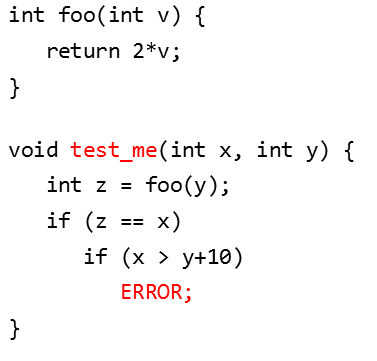
\includegraphics[width=0.5\linewidth]{images/dse1.png}
%\end{frame}
%
%\begin{frame}{Ví dụ: Cách thức hoạt động của DSE}
%\centering
%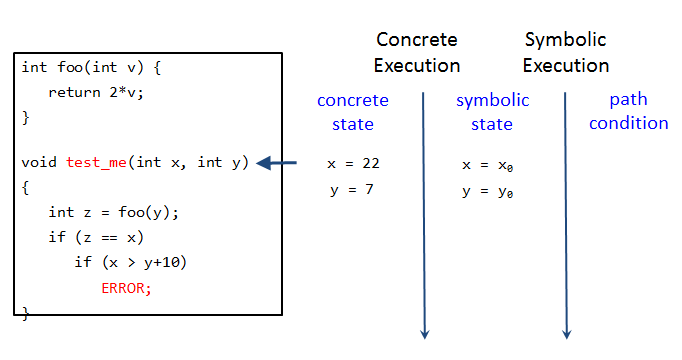
\includegraphics[width=0.9\linewidth]{images/dse11.png}
%\end{frame}
%
%\begin{frame}{Ví dụ: Cách thức hoạt động của DSE}
%\centering
%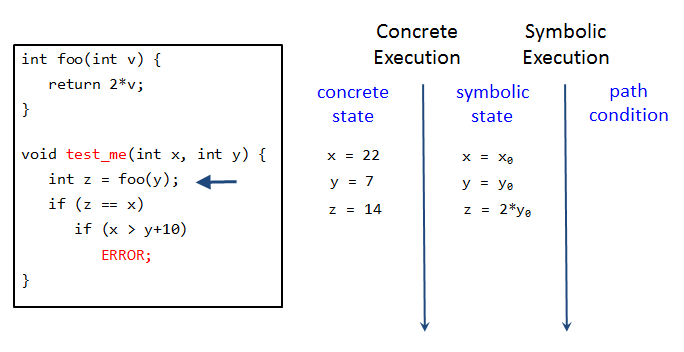
\includegraphics[width=0.9\linewidth]{images/dse12.png}
%\end{frame}
%
%\begin{frame}{Ví dụ: Cách thức hoạt động của DSE}
%\centering
%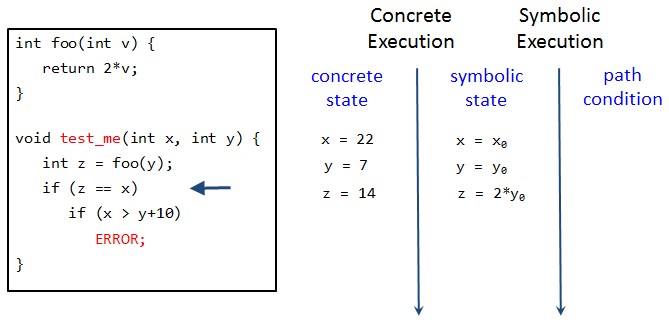
\includegraphics[width=0.9\linewidth]{images/dse121.png}
%\end{frame}
%
%\begin{frame}{Ví dụ: Cách thức hoạt động của DSE}
%\centering
%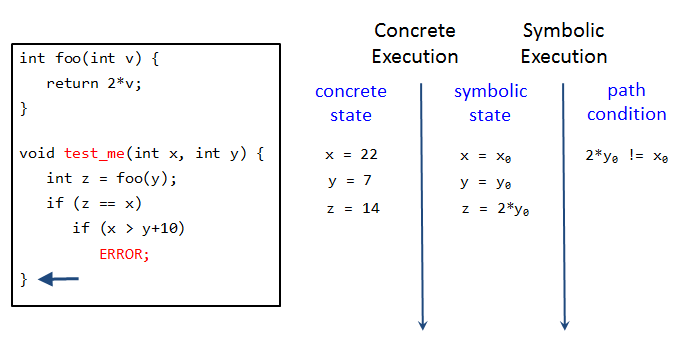
\includegraphics[width=0.9\linewidth]{images/dse13.png}
%\end{frame}
%
%\begin{frame}{Ví dụ: Cách thức hoạt động của DSE}
%\centering
%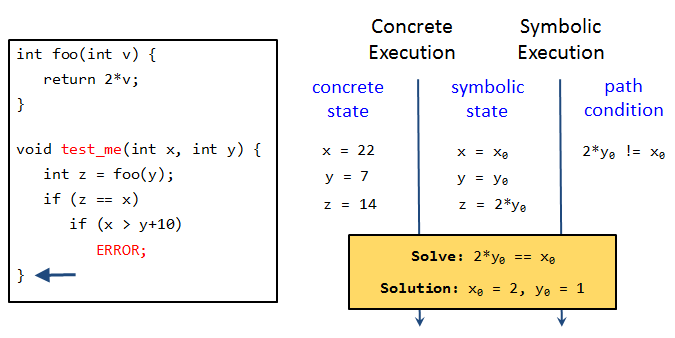
\includegraphics[width=0.9\linewidth]{images/dse2.png}
%\end{frame}
%
%\begin{frame}{Ví dụ: Cách thức hoạt động của DSE}
%\centering
%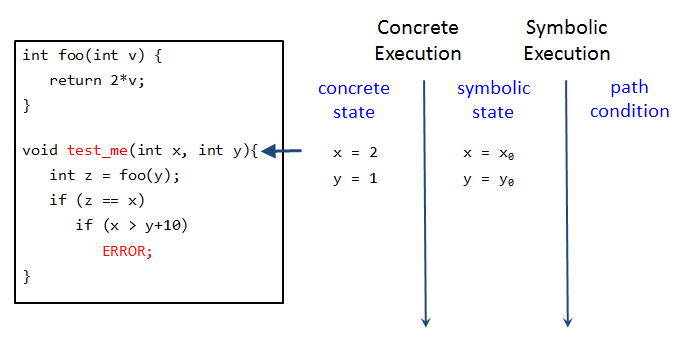
\includegraphics[width=0.9\linewidth]{images/dse21.png}
%\end{frame}
%
%\begin{frame}{Ví dụ: Cách thức hoạt động của DSE}
%\centering
%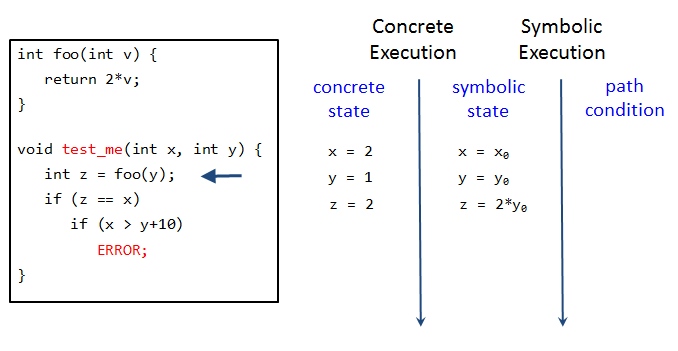
\includegraphics[width=0.9\linewidth]{images/dse22.png}
%\end{frame}
%
%\begin{frame}{Ví dụ: Cách thức hoạt động của DSE}
%\centering
%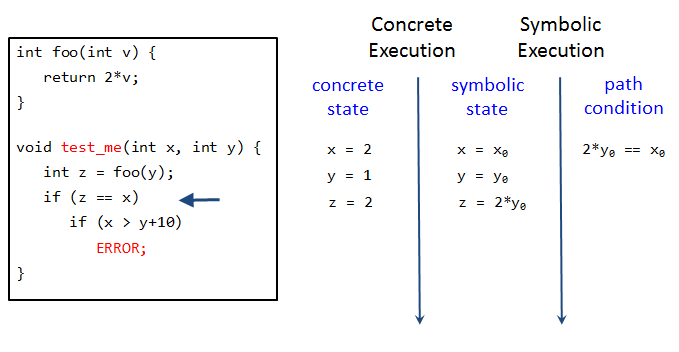
\includegraphics[width=0.9\linewidth]{images/dse23.png}
%\end{frame}
%
%\begin{frame}{Ví dụ: Cách thức hoạt động của DSE}
%\centering
%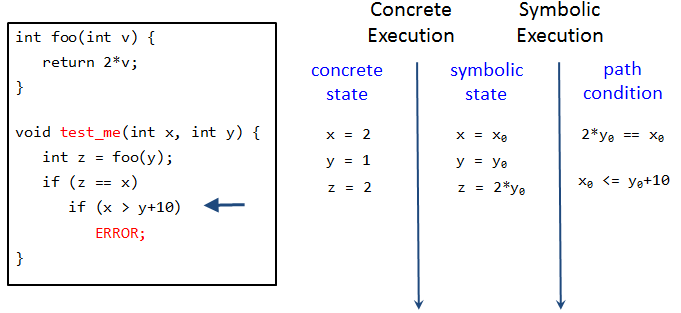
\includegraphics[width=0.9\linewidth]{images/dse231.png}
%\end{frame}
%
%\begin{frame}{Ví dụ: Cách thức hoạt động của DSE}
%\centering
%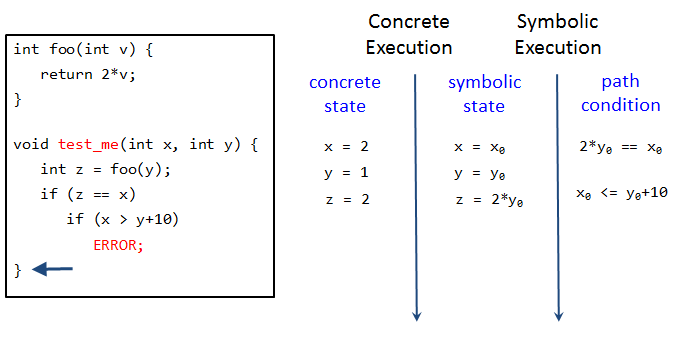
\includegraphics[width=0.9\linewidth]{images/dse24.png}
%\end{frame}
%
%\begin{frame}{Ví dụ: Cách thức hoạt động của DSE}
%\centering
%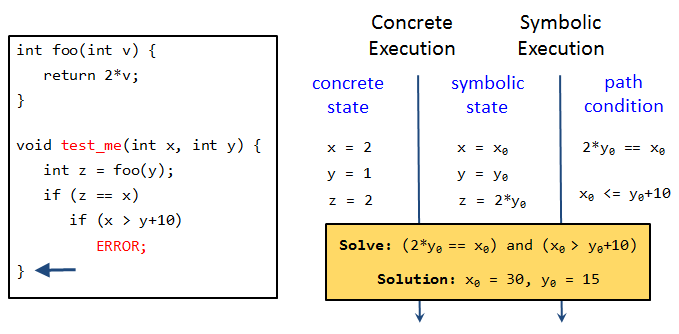
\includegraphics[width=0.9\linewidth]{images/dse3.png}
%\end{frame}
%
%\begin{frame}{Ví dụ: Cách thức hoạt động của DSE}
%\centering
%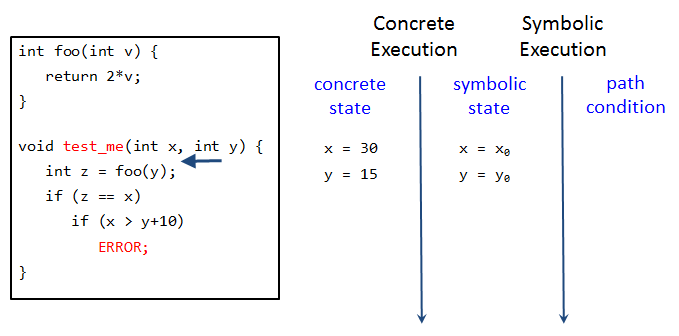
\includegraphics[width=0.9\linewidth]{images/dse31.png}
%\end{frame}
%
%\begin{frame}{Ví dụ: Cách thức hoạt động của DSE}
%\centering
%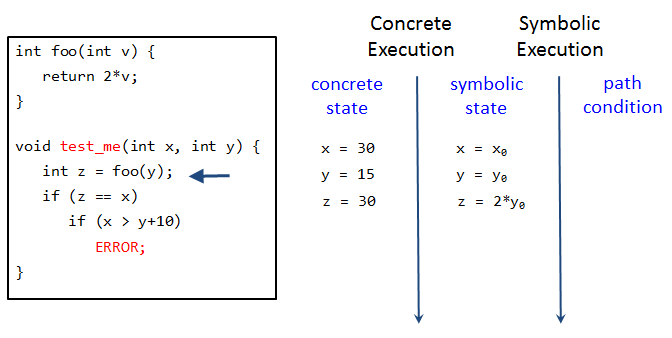
\includegraphics[width=0.9\linewidth]{images/dse32.png}
%\end{frame}
%
%\begin{frame}{Ví dụ: Cách thức hoạt động của DSE}
%\centering
%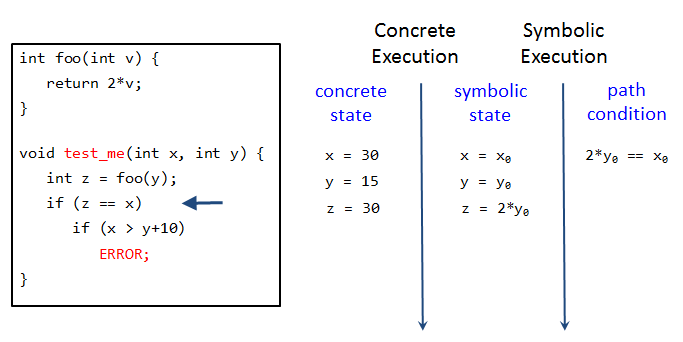
\includegraphics[width=0.9\linewidth]{images/dse33.png}
%\end{frame}
%
%\begin{frame}{Ví dụ: Cách thức hoạt động của DSE}
%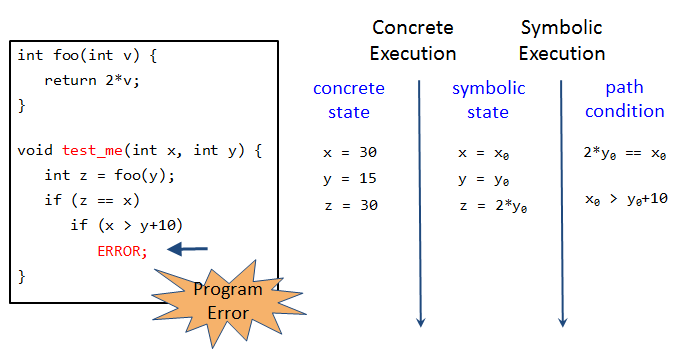
\includegraphics[width=0.9\linewidth]{images/dse4.png}
%\pause
%\\Sau $ 3 $ lần thực thi chương trình DSE đã tạo ra được các giá trị đầu vào $ \{x = 22, y = 7\} $, $ \{x = 2, y = 1\} $ và $ \{x = 30, y = 15\} $
%\end{frame}

\subsection{Hành vi của chương trình}
\subsubsection*{Thực thi chương trình}
\label{lb:TTCT}
\begin{frame}{Hành vi của chương trình}
\begin{block}{\ref{lb:TTCT}. Thực thi chương trình}
Thực thi một chương trình là sự tương ứng mỗi giá trị vào với một giá trị ra.
\end{block}

\begin{exampleblock}{Định nghĩa: Thực thi chương trình}
Cho $P$ là một chương trình, $I$ là tập hợp các trị đầu vào của $P$
và $O$ là tập hợp các giá trị đầu ra của $P$. Thực thi chương trình
P là ánh xạ:
\[exec: P \times I \rightarrow O.\]
Với giá trị đầu vào $i \in I$, sau khi thực thi chương trình $P$ trên
$i$ ta thu được giá trị đầu ra tương ứng $o \in O, o = exec(P, i)$.
\end{exampleblock}
\end{frame}

\subsubsection*{Tương đương về hành vi}
\label{lb:TDVHV}
\begin{frame}{Hành vi của chương trình}
\begin{block}{\ref{lb:TDVHV}. Tương đương về hành vi}
Hai chương trình được gọi là tương đương với nhau về hành vi nếu chúng
biến đổi cùng một giá trị vào thành cùng một giá trị ra đối với mọi
giá trị trên miền vào
\end{block}
\begin{exampleblock}{Ví dụ:}
\begin{minipage}[t]{0.45\linewidth}
	\lstinputlisting[basicstyle=\tiny, caption =
	{Chương trình $ P_{1} $}]{SwitchCase.cs}
\end{minipage}%
\hfill\vrule\hfill
\begin{minipage}[t]{0.45\linewidth}
	\lstinputlisting[basicstyle=\tiny, caption =
	{Chương trình $ P_{2} $}]{IfElse.cs}
\end{minipage}%	
\end{exampleblock}
\end{frame}

\subsubsection*{Khác biệt về hành vi}
\label{lb:KBVHV}
\begin{frame}{Hành vi của chương trình}
\begin{block}{\ref{lb:KBVHV}. Sự khác biệt về hành vi}
Hai chương trình có hành vi khác nhau nếu chúng có miền giá trị đầu vào khác nhau, hoặc
có một vài giá trị vào làm cho thực thi của chúng khác nhau.
\end{block}
\begin{exampleblock}{Ví dụ:}
\begin{minipage}[t]{0.45\linewidth}
	\lstinputlisting[basicstyle=\tiny, caption={Hành vi $ P_{1} $}, label={KBHV1}]{Khac_biet_HV_1.cs}
\end{minipage}%
\hfill\vrule\hfill
\begin{minipage}[t]{0.45\linewidth}
	\lstinputlisting[basicstyle=\tiny, caption={Hành vi $ P_{2} $}, label={KBHV2}]{Khac_biet_HV_2.cs}
\end{minipage}%
\end{exampleblock}
\end{frame}

\subsubsection*{Độ tương tự về hành vi}
\label{lb:DTTVHV}
\begin{frame}{Hành vi của chương trình}
\begin{block}{\ref{lb:DTTVHV}. Độ tương tự về hành vi}
Hai chương trình không tương đương nhau về hành vi, nghĩa là có sự 
khác biệt về hành vi giữa chúng, thì ta cần biết mức độ tương tự 
giữa chúng là bao nhiêu.
\end{block}
\begin{exampleblock}{Ví dụ:}
	\begin{minipage}[t]{0.45\linewidth}
		\lstinputlisting[basicstyle=\tiny, caption = {Chương trình $P_{1}$}]{TuongTu_HV_1.cs}
	\end{minipage}%
	\hfill\vrule\hfill
	\begin{minipage}[t]{0.45\linewidth}
		\lstinputlisting[basicstyle=\tiny, caption = {Chương trình $P_{2}$}]{TuongTu_HV_2.cs}
	\end{minipage}%	
\end{exampleblock}
Độ tương tự về hành vi: $|E| / |\texttt{int}|$, trong đó $E = [0,100] \cup \{-1\}$
\end{frame}

\subsection{Một số phép đo độ tương tự hành vi}
\label{subsec:MSPD}
\subsubsection*{Lẫy mẫu ngẫu nhiên}
\label{subsubsec:RS}
\begin{frame}{Một số phép đo độ tương tự hành vi}
\begin{block}{\ref{subsubsec:RS}. Lấy mẫu ngẫu nhiên}
\begin{itemize}
\item Lấy ngẫu nhiên một số giá trị trên miền vào
\item Tính số lượng giá trị mà ở đó hai chương trình thực thi giống nhau, 
từ đó tính mức độ tương tự
\item Gọi phép đo độ tương tự theo phương pháp này là \emph{Phép đo RS - Random Sampling}
\end{itemize}
\end{block}
\pause
%\begin{definition}[Phép đo RS]
%  \label{def:RS-sim}
%  Cho $P_{1}$ và $P_{2}$ là hai chương trình có cùng miền giá trị đầu
%  vào $I$, $I_{s}$ là tập con ngẫu nhiên của $I$, $I_{a}$ là tập con
%  $I_{s}$ sao cho $exec(P_{1}, I_a) = exec(P_{2}, I_a)$ và
%  $\forall j \in I_{s} \setminus I_{a}$, thì
%  $exec(P_{1}, j) \neq exec(P_{2}, j)$. Độ tương tự về hành vi giữa
%  hai chương trình theo phép đo RS được định nghĩa là
%  $M_{RS}(P_{1}, P_{2}) = \left|I_{a}\right| \diagup
%  \left|I_{s}\right| $.
%\end{definition}
\end{frame}

\begin{frame}{Một số phép đo độ tương tự hành vi}
\begin{algorithm}[H]
\begin{algorithmic}[1]
\item $P_{1}, P_{2}:$ Là hai chương trình cần đo độ tương tự
\item $I$: Miền giá trị đầu vào của $P_{1}, P_{2}$
\item Set $I_{s} = Random(I)$ 
\item Set $I_{a} = \emptyset$
\FOR {$i \in I_s$}
    \IF{ ($exec(P_{1}, i) = exec(P_{2}, i)$) } 
	\STATE $I_{a} = I_{a} \cup i$
\ENDIF
\ENDFOR
\item $M_{RS}(P_{1}, P_{2}) = \left|I_{a}\right| \diagup
    \left|I_{s}\right| $.
\end{algorithmic}
\caption{Thuật toán phép đo RS }
\label{alg:seq}
\end{algorithm}
\end{frame}

\begin{frame}{Một số phép đo độ tương tự hành vi}
\begin{exampleblock}{Ví dụ: Hạn chế của phép đo RS}
	\begin{minipage}[t]{0.45\linewidth}
	\lstinputlisting[basicstyle=\small, label={RS1},caption = {Chương trình
		$P_{1}$}]{RS1.cs}
	\end{minipage}%
	\hfill\vrule\hfill
	\begin{minipage}[t]{0.45\linewidth}
		\lstinputlisting[basicstyle=\small, label={RS2}, caption = {Chương trình
			$P_{2}$}]{RS2.cs}
	\end{minipage}% 
\end{exampleblock}
\begin{itemize}
	\item $P_{1}$ có thể sẽ không thực thi nhánh \texttt{(x == "XYZ")}
	\item Độ bao phủ của dữ liệu sinh ngẫu nhiên không cao.
\end{itemize}
\end{frame}

\subsubsection*{DSE trên chương trình tham chiếu}
\label{subsubsec:SSE}
\begin{frame}{Một số phép đo độ tương tự hành vi}
\begin{block}{\ref{subsubsec:SSE}. DSE trên chương trình tham chiếu}
\begin{itemize}
	\item Khắc phục nhược điểm của phép đo RS bằng cách áp dụng kỹ thuật
	DSE để tăng độ bao phủ của tập dữ liệu thử
	\item Chỉ cần dựa vào chương trình tham chiếu để xác
	định tập dữ liệu thử.
	\item Gọi tắt là SSE (\emph{Single program Symbolic Execution})
\end{itemize}
\end{block}
%\pause
%\begin{definition}[Phép đo SSE]
%  \label{def:sse}
%  Cho $P_{1}$ và $P_{2}$ là hai chương trình có cùng miền giá trị đầu
%  vào $I$, trong đó $P_{1}$ là chương trình tham chiếu. Gọi $I_{s}$ là
%  tập các giá trị đầu vào được tạo bởi DSE trên $P_{1}$, và
%  $I_{a} \subseteq I_s$ là tập con lớn nhất của $I_{s}$ sao cho
%  $exec(P_{1}, I_a) = exec(P_{2}, I_a)$ và
%  $\forall j \in I_{s} \setminus I_{a}, exec(P_{1}, j) \neq
%  exec(P_{2}, j)$. Độ tương tự về hành vi giữa hai chương trình dùng
%  phép đo SSE được định nghĩa là
%  $M_{SSE}(P_{1}, P_{2}) = \left|I_{a}\right| \diagup
%  \left|I_{s}\right| $.
%\end{definition}
\end{frame}

\begin{frame}{Một số phép đo độ tương tự hành vi}
\begin{algorithm}[H]
\caption{Thuật toán phép đo SSE}
\begin{algorithmic}[1]
  \item $P_{1}, P_{2}:$ hai chương trình cần đo tương tự, $P_1$ là chương trình tham chiếu
  \item $I$: Miền giá trị đầu vào của $P_{1}, P_{2}$
  \item $I_{s}$: Tập đầu vào của $P_{1}$ theo DSE
  \item Set $I_{s} = DSE(P_{1})$  
  \item Set $I_{a} = \emptyset$
    \FOR{ ($i \in I_{s}$) }
    \IF{ ($exec(P_{1}, i) = exec(P_{2}, i)$) } 
	\STATE $I_{a} = I_{a} \cup i$
    \ENDIF
    \ENDFOR
  \item
    $M_{SSE}(P_{1}, P_{2}) = \left|I_{a}\right| \diagup
    \left|I_{s}\right| $.
  \end{algorithmic}
\end{algorithm}
\end{frame}

\begin{frame}{Một số phép đo độ tương tự hành vi}
\begin{exampleblock}{Ví dụ: Hạn chế của phép đo SSE}
	\begin{minipage}[t]{0.45\linewidth}
		\lstinputlisting[basicstyle=\tiny, label={SSE1}, 
		caption = {Chương trình tham chiếu $P_{1}$}]{SSE1.cs}
	\end{minipage}%
	\hfill\vrule\hfill
	\begin{minipage}[t]{0.45\linewidth}
		\lstinputlisting[basicstyle=\tiny, label={SSE2}, 
		caption = {Chương trình cần thực thi $P_{2}$}]{SSE2.cs}
	\end{minipage}%
	\begin{itemize}
		\item $DSE(P_{1})$ ta có tập giá trị đầu vào là $(0, 1)$.  
		$M_{SSE}(P_{1}, P_{2}) = 1$
		\item Nhánh $ (x == 2) $ của chương trình $ P_{2} $ không được thực thi
	\end{itemize}
\end{exampleblock}
\end{frame}

\subsubsection*{DSE trên chương trình hợp thành}
\label{subsubsec:PSE}
\begin{frame}{Một số phép đo độ tương tự hành vi}
\begin{block}{\ref{subsubsec:PSE}. DSE trên chương trình hợp thành}
\begin{itemize}
	\item Giải quyết giới hạn của phép đo SSE
	\item Xây dựng một chương trình hợp thành kết hợp cả hai
	\item Sử dụng kỹ thuật DSE trên chương trình hợp thành 
	để tăng độ bao phủ của tập dữ liệu thử
	\item Gọi tắt là phép đo PSE (Paired
	program Symbolic Execution)
\end{itemize}
\end{block}
%\pause
%\begin{definition}[Chương trình hợp thành]
%  \label{def:combination}
%  Cho $P_1$ và $P_2$ là hai chương trình có cùng miền vào $I$, trong đó
%  $P_1$ là chương trình tham chiếu. Hợp thành của hai chương trình là
%  một chương trình mới $P_c = P_1 \oplus P_2$ có dạng
%  $assert(exec(P_{1}, I) = exec(P_{2}, I))$, trong đó $assert(\dots)$
%  là hàm đánh giá nhận vào một biểu thức điều kiện và đánh giá xem
%  biểu thức đó đúng hay sai. Ký hiệu $exec(P_c,i) = \top$ để chỉ
%  chương trình hợp thành $P_c$ thỏa hàm đánh giá, cũng có nghĩa là hai
%  chương trình thành phần thực thi giống nhau trên đầu vào $i$.
%\end{definition}
\end{frame}
\begin{frame}{Một số phép đo độ tương tự hành vi}
\begin{algorithm}[H]
	\caption{Thuật toán phép đo PSE}
	\begin{algorithmic}[1]
   \item $P_{1}, P_{2}$: hai chương trình cần đo tương tự, $P_1$ là
     chương trình tham chiếu
   \item $I$: Miền giá trị đầu vào của $P_{1}, P_{2}$
   \item $P_{3} = P_1 \oplus P_2$
   \item $I_{s}$: Tập đầu vào của $P_{3}$ theo DSE
   \item Set $I_{s} = DSE(P_{3})$ 
   \item Set $I_{a} = \emptyset$ 
   		\FOR{$i \in I_{s}$}
     	\IF{($exec(P_{1}, i) = exec(P_{2}, i)$) } 
     	\STATE $I_{a} = I_{a} \cup i$ 
     	\ENDIF 
     	\ENDFOR
   \item $M_{PSE}(P_{1}, P_{2}) = \left|I_{a}\right| \diagup
     \left|I_{s}\right| $.
   \end{algorithmic}
 \end{algorithm}
\end{frame}

\begin{frame}{Một số phép đo độ tương tự hành vi}
\begin{exampleblock}{Ví dụ: Phép đo PSE}
	\begin{minipage}[t]{0.3\linewidth}
	\lstinputlisting[basicstyle=\tiny, caption={Chương trình hợp thành}, label={lst:PSE}]{PSE3.cs}
	\end{minipage}%
	\hfill\vrule\hfill
	\begin{minipage}[t]{0.3\linewidth}
		\lstinputlisting[basicstyle=\tiny,caption={Chương trình tham chiếu $ T1 $}, label={lst:PSE-T1}]{PSE1.cs}
	\end{minipage}%
	\hfill\vrule\hfill
	\begin{minipage}[t]{0.3\linewidth}
	\lstinputlisting[basicstyle=\tiny,caption={Chương trình cần tính $ T2 $}, label={lst:PSE-T2}]{PSE2.cs}
\end{minipage}%
\end{exampleblock}
\begin{itemize}
	\item DSE(HT) kết quả thu được $ 0, 1, 2 $
	\item Với giá trị bằng $ 0 $, $exec(P_{1}, 0) = exec(P_{2}, 0)$
	\item $  M_{PSE}(P_{1}, P_{2}) = 0.33 $
\end{itemize}
\end{frame}